\documentclass[final,3p,times,number]{elsarticle}
\usepackage[utf8]{inputenc}
\usepackage{graphicx}
\usepackage{booktabs}
\usepackage{array}
\usepackage{tabularx}
\usepackage{amsmath}
\usepackage{amssymb}
\usepackage{placeins}
\usepackage{float}
\usepackage[font=small,skip=6pt]{caption}
\usepackage{microtype}
\usepackage{tikz}
\usepackage{url}
\usetikzlibrary{arrows.meta,positioning,shapes.geometric}
\urlstyle{same}
\captionsetup{labelfont=bf,justification=centering}
\emergencystretch=2em
\newcolumntype{Y}{>{\raggedright\arraybackslash}X}
\setlength{\textfloatsep}{6pt plus 1pt minus 2pt}
\setlength{\floatsep}{6pt plus 1pt minus 2pt}
\setlength{\intextsep}{6pt plus 1pt minus 2pt}
\renewcommand{\arraystretch}{1.08}
\raggedbottom
\setcounter{topnumber}{5}
\setcounter{bottomnumber}{2}
\setcounter{totalnumber}{6}
\renewcommand{\topfraction}{0.95}
\renewcommand{\bottomfraction}{0.85}
\renewcommand{\textfraction}{0.05}
\renewcommand{\floatpagefraction}{0.85}
\journal{Engineering Applications of Artificial Intelligence}


\begin{document}
\begin{frontmatter}

\title{Brain Tumour Detection and Classification: A Comparative Study of Advanced Deep Learning Models}

\author[vit]{Parth Mital\corref{cor1}}
\author[vit]{Ved Lawand}
\author[vit]{Biji C. L.}
\cortext[cor1]{Corresponding author. Email addresses: parth.mital2023@vitstudent.ac.in, ved.lawand2023@vitstudent.ac.in, biji.cl@vit.ac.in}

\affiliation[vit]{organization={School of Computer Science and Engineering, Vellore Institute of Technology},
city={Vellore},
country={India}}

\begin{abstract}
Brain tumour diagnosis from magnetic resonance imaging (MRI) is clinically important, but manual interpretation is time consuming, variable, and dependent on specialist expertise. This study benchmarks nine deep learning architectures for tumour detection and subtype classification into glioma, meningioma, and pituitary tumours. The comparison covers classical convolutional neural networks (CNNs), efficient CNNs, and transformer or hybrid transformer models under a common preprocessing, training, and evaluation protocol. Perceptual hash based deduplication was applied before splitting the multiclass dataset, reducing 5,828 images to 4,705 unique samples; binary detection used 3,253 images. All models used ImageNet pretraining, AdamW optimisation, cosine annealing, and mixed precision training. CoaTNet-0 and EfficientNetB0 achieved the best binary detection accuracy of 99.59\%, while InceptionV3 achieved 99.39\% with an area under the receiver operating characteristic curve (AUC) of 1.0000. InceptionV3 and Swin Base achieved the best multiclass accuracy of 98.58\%. EfficientNetB0 gave the best accuracy-efficiency balance, reaching 97.59\% multiclass accuracy with 5.3 million parameters.
\end{abstract}

\begin{keyword}
Brain tumour detection, deep learning, convolutional neural networks, vision transformers, medical image classification, MRI, transfer learning
\end{keyword}

\end{frontmatter}


\section{Introduction}

Brain tumours constitute the abnormal proliferation of cells either in the brain or the central nervous system. Whether benign or malignant, brain tumours represent serious threats because of their location in the limited skull cavity and the important functions of the brain. According to American Brain Tumour Association, about 90,000 people are estimated to have primary brain tumours each year in the USA alone, while the global scenario is similar with respect to incidence. The exact prevalence in India, however, is not fully documented. Nonetheless, in the major metropolitan cities like Mumbai, Delhi, Bangalore, and Chennai, the tertiary care hospitals report thousands of patients with primary brain tumours each year. Three major forms of primary brain tumours include: (i) glioma, which is formed from glial cells and constitutes 30\% of total brain tumours; (ii) meningioma, which develops in the meningeal layers of the brain, is usually benign in nature, and (iii) pituitary tumours that grow in the pituitary gland causing hormonal problems \cite{ref1,ref2}.

MRI or Magnetic Resonance Imaging is used nowadays as the main non-invasive technique for brain tumours detection and classification. In comparison to the traditional CT imaging, MRI gives much better soft tissue contrast without utilising any ionising radiation. Moreover, MRI allows getting pictures in different directions and using different types of contrasts -- namely, T1-weighted, T2-weighted, FLAIR, and diffusion-weighted. This is extremely important for tumour location, volume, margins, oedema, and adjacent vital structures determination. At the same time, analysis of MRI studies raises a number of problems that cannot be ignored. Firstly, it takes a lot of time for examination -- the complete brain MRI study may include hundreds of sections, while it takes a specialist radiologist 15-30 minutes to make a correct diagnosis \cite{ref20,ref21}. Secondly, inter- and intra-observer variabilities should be noted; i.e. there is no guarantee that radiologists will interpret the results of MRI in the same way. Thirdly, lack of knowledge in neuroradiology can become an obstacle for correct image interpretation. Finally, there is no enough specialists in the rural and semi-urban regions of India because of their poor radiologist/population ratio.

The introduction of deep learning technology has transformed the field of medical imaging analysis in the last ten years. The models based on deep learning, especially convolutional neural networks (CNN), have the ability to learn hierarchical representation of the visual features directly from pixel inputs without the need for manual feature extraction. Thus, the use of these models enables automatic, efficient, and consistent tumour detection from brain MRIs. Convolutional neural networks have become popular among researchers working in this area, with well-performing models like ResNet, VGG, DenseNet, Inception, EfficientNet, and MobileNet setting benchmarks on image classification tasks. Recently, researchers started exploring transformer models for computer vision problems, which were initially used in natural language processing. These transformer-based models include ViT, Swin Transformer, and CoaTNet. This line of research provides an alternate way of representing global information in the images using self-attention mechanism, and it might be of particular use in medical imaging, especially when understanding the relation between a tumour and the surrounding anatomical structures \cite{ref28}, \cite{ref29}, \cite{ref30}, \cite{ref32}.

Although several research works have separately proved the efficiency of deep learning architectures in the case of detecting and classifying brain tumours, there is still an insufficient number of comparative investigations performed across several architectural groups using the same sets of parameters. The lack of comparative analysis poses serious challenges in choosing the required models, since each research employs separate databases, preprocessing procedures, data augmentation approaches, as well as assessment techniques, which makes it quite problematic to compare the results received from various scientific studies. For example, it is impossible to say which performance indicator is better when one work indicates an accuracy of 99\% based on a small and homogeneous database, whereas another one gives 97\% accuracy based on a larger and heterogeneous one.

Even though there exist numerous studies confirming the efficiency of deep learning models for detection and classification of brain tumours, however, there are only a few comparative studies analysing efficiency of several different architectural designs with the use of the same parameters. The problem with comparative analysis hinders greatly in selecting the right model, as every study uses its own particular database, preprocessing method, augmentation, and evaluation technique, making comparison of results obtained in various scientific research almost impossible. To illustrate, it is not possible to decide which indicator is more accurate in a case where one study shows 99\% accuracy but uses small homogenous database, while the other gives 97\% but uses a large heterogeneous one.

Numerous papers make the mistake of containing images that are near-duplicates or duplicates across the training, validation, and test splits when using publicly available datasets from multiple sources. This results in a highly inaccurate assessment of the performance, causing a significant increase in reported performance figures compared to the actual ability of a model to generalise. Once a neural network or other machine learning model has been shown a particular image (or one that is very similar) in training, any further performance results for that image will be a reflection of memory and not true learning. The problem of near-duplicate images is especially critical within brain tumour research, since most publicly available datasets come from common origins, like the Cheng dataset or the Figshare dataset. Most papers that discuss this problem use simple exact-matching techniques that rely either on the file name or the cryptographic hash of an image. However, exact-matching techniques fail to detect even simple modifications such as changing the size of an image, recompressing it, rotating it slightly, or changing its contrast.

It is important to emphasise the clinical significance of brain tumour diagnosis being correctly established. The potential consequences of late or misdiagnosis include limited treatment alternatives, poor prognosis, higher healthcare expenditures, and significantly diminished quality of life for both patients and their families. The implementation of automated systems with equal or superior accuracy to humans may bring about several advantages: faster diagnosis due to prompt preliminary diagnosis; decision-making support where there are no experienced radiologists to make such decisions; uniformity of diagnoses made due to the lack of inter-reader variation; as well as freeing up the work of radiologists who should only attend to challenging cases requiring an expert opinion \cite{ref13,ref14}. This problem has especially high significance in India. Recent workforce studies indicate that there is only one radiologist per 100,000 people in the country, although the optimal rate would be one per 10,000, which implies a shortage of almost 90\%. Consequently, most district and community healthcare facilities have no radiologists at all. In addition, even in places where radiologists are available, the speciality of neuroradiology is uncommonly trained, and brain tumours can only be accurately diagnosed in very specialised tertiary care hospitals. Thus, automated diagnostic systems would be especially important for tackling the problem of medical accessibility in India, which ranges from urban slums to rural areas, such as the ones found in Uttar Pradesh, Bihar, Madhya Pradesh, and North-Eastern regions \cite{ref27}.

The purpose of this paper is to achieve several objectives. Firstly, the implementation of nine deep learning models that are varied in nature from traditional convolutional neural networks (ResNet50, VGG16, DenseNet121) to more efficient networks (EfficientNetB0, MobileNetV3-Large, InceptionV3) as well as transformers (ViT-B/16, Swin Transformer Base, CoaTNet-0). Secondly, establishing a common testing protocol based on the use of the same train-test splits, similar preprocessing approaches including perceptual hashing for deduplication of images, and comparable hyper-parameters for all of the models. Thirdly, the assessment of models' performance by the means of clinical performance metrics such as accuracy, AUC-ROC score, cross-entropy loss function, and efficiency metrics like parameter count and training time. Fourthly, the exploration of architectural trends in the field of brain tumour analysis in order to find out whether residual, dense, multi-scale, attention-based designs, or neural architecture search can improve performance. Fifthly, evidence-based recommendations on the model selection for different scenarios based on the trade-off between accuracy and efficiency.

The rest of this paper is structured as follows. Section 2 reviews existing studies in conventional machine learning, CNNs, transformers, and brain tumour classification to identify the contribution of this work. Section 3 describes dataset preparation, perceptual hash based deduplication, hierarchical routing, preprocessing, augmentation, model architecture choices, and experimental settings. Section 4 presents and discusses the binary detection and multiclass classification results. Section 5 discusses limitations and future work. Section 6 addresses ethical implications for clinical deployment, particularly in India and other resource-constrained settings. Section 7 concludes the study.

\section{Literature Review}

Previous works on automated brain tumour recognition were based on feature engineering followed by machine learning classifiers. Such works have used texture descriptors like GLCM and LBP; wavelets like DWT; morphological features related to shape, size, and boundary; and classifiers like SVM, Random Forests, and k-NN \cite{ref2}, \cite{ref3}. In their work, Zacharaki et al. \cite{ref1} obtained around 85\% accuracy using texture features and SVM classifier on a small set of 80 images for tumour type recognition. Cheng et al. \cite{ref5} suggested a tumour region enhancement approach that yielded 90\% accuracy using intensity, texture, and shape features along with SVM classifier on 3064 MRI images. Although promising, such methods faced challenges due to the limitations of feature engineering, inability to generalise to different datasets, and lack of automatic learning of hierarchical structures.

The revolution by AlexNet in 2012 propelled the implementation of deep learning in medical imaging applications. The successive CNN models have improved their performances by introducing better architectures. Residual connections were incorporated into CNN models, thereby making it possible to train very deep networks by solving the vanishing gradients issue by He et al. \cite{ref6}. ResNet50 became a standard model for medical image classification with the reports of 95-98\% accuracy for classifying brain tumours. Using transfer learning technique on ResNet50 model, Seetha and Raja \cite{ref12} achieved an accuracy of 97.5\% for the classification of 253 MRI brain images. The researchers demonstrated the improvement in model performances by incrementing its depth while keeping small convolutional filters ($3\times 3$). However, due to its huge parameters (138 million), VGG16 is computationally intensive and vulnerable to over-fitting when applied to small medical datasets. For instance, in their work, Khan et al. \cite{ref23} reported 98.69\% accuracy using VGG16 with the number of samples of 3,064. Huang et al. \cite{ref9} introduced densely connected layers where each layer receives input from all previous layers. Consequently, DenseNet121 became more efficient with parameter count while having better performance in medical imaging tasks (accuracies of 96-98\%). Szegedy et al. \cite{ref7} presented parallel convolutions with varying dimensions ($1\times 1$, $3\times 3$, $5\times 5$) that allowed the model to learn from multi-level features. InceptionV3 was able to reach 97.5\% accuracy in classifying brain tumours, as cited by Deepak and Ameer \cite{ref15}. Moreover, Rehman et al. \cite{ref25} obtained a high classification rate of 99.34\% accuracy via transfer learning. Tan and Le \cite{ref18} introduced a method for scaling up the network dimensionality (depth, width, and resolution) using neural architecture search to obtain better accuracy using much fewer parameters than other models. EfficientNetB0 uses only 10 $\times$ the number of parameters used by ResNet50. Furthermore, Howard et al. \cite{ref19} created lightweight neural networks based on depth-wise separable convolutions for mobile and edge devices.

Dosovitskiy et al. \cite{ref28} leveraged transformer models for visual tasks by framing images as patch sequences ($16\times 16$ pixels). The ViT-B/16 variant performed comparably with CNNs on large-scale data sets (ImageNet, JFT-300M) but needed significant pre-training and exhibited drawbacks on small medical data sets because of a lack of built-in inductive biases. Liu et al. \cite{ref29} proposed hierarchical transformers using shifted windows to process images efficiently at multiple scales without sacrificing linear complexity concerning image resolution. Swin Transformers performed impressively on ImageNet data sets. They have been investigated for their applications in medical image processing too. The hierarchical window attention in Swin Transformers enables the model to learn about the local boundaries of tumours and the overall structure from the MRIs. CoaTNet is an example by Xu et al. \cite{ref30}, which employs convolution and attention simultaneously in one model.

Recent studies applying these architectures to brain tumour detection include the comparative summary presented in Table~\ref{tab:existing-studies}.

\begin{table}[htbp]
\centering
\caption{Comparison of Existing Studies for Brain Tumour Detection}
\label{tab:existing-studies}
\begin{tabularx}{\textwidth}{@{}YYccc@{}}
\toprule
Study & Model & Dataset Size & Task & Accuracy \\
\midrule
Talo et al. (2019) \cite{ref16} & ResNet50 & 253 & Binary & 95.23\% \\
Khan et al. (2020) \cite{ref23} & VGG16 & 3,064 & Binary & 98.69\% \\
Noreen et al. (2020) \cite{ref24} & DenseNet121 & 3,064 & Binary & 99.51\% \\
Rehman et al. (2020) \cite{ref25} & InceptionV3 & 3,064 & Binary & 99.34\% \\
Ghassemi et al. (2020) \cite{ref26} & EfficientNet & 3,064 & Binary & 98.87\% \\
Cheng et al. (2015) \cite{ref5} & SVM + Features & 3,064 & Multiclass & 90.00\% \\
Deepak and Ameer (2019) \cite{ref15} & InceptionV3 & 3,064 & Multiclass & 97.50\% \\
\bottomrule
\end{tabularx}
\end{table}

However, several open issues remain. Cross-architecture comparison is difficult because many papers evaluate only two or three models. Dataset heterogeneity creates further obstacles because train-test splits, preprocessing steps, and evaluation protocols differ across studies. Transformer-based models are still under-represented in public brain tumour classification comparisons. Reproducibility is also limited because source code, exact splits, and pretrained weights are not always released. Incomplete deduplication is another gap because many studies do not consider duplicate and near-duplicate images in merged public datasets. This paper addresses these gaps by evaluating nine architectures under the same conditions, combining datasets from multiple public sources, applying perceptual hash based deduplication, comparing CNN and transformer families, and presenting both binary and multiclass task results under standardised evaluation schemes.

\section{Methods and Materials}

\subsection{Hierarchical Workflow}

The detection and classification system is presented as a hierarchy rather than as a single flat classifier. The input stage first records available modality metadata when it is present. In the two-dimensional public datasets used in the detection and classification notebooks, reliable modality labels are not available for every image; therefore, this stage is treated as input handling rather than as a trained modality classifier. The next stage performs binary tumour detection. Only tumour-positive cases proceed to subtype classification into glioma, meningioma, and pituitary tumour classes. This hierarchy follows the clinical interpretation order and prevents subtype prediction from being applied to tumour-negative images. The staged presentation is consistent with hierarchical brain image interpretation workflows described in recent medical image classification literature \cite{ref33}.

This hierarchical presentation is important because the two classification schemes answer different clinical questions. Binary detection estimates whether a tumour-like abnormality is visible in the scan, while subtype classification is meaningful only after a tumour-positive decision has already been made. A flat four-class presentation that combines non-tumour, glioma, meningioma, and pituitary cases would not reflect this order and would also make the subtype model responsible for rejecting normal images that were not part of its training objective. Separating the tasks therefore keeps the experimental interpretation aligned with the notebooks: the binary detector is evaluated as the routing model, and the multiclass model is evaluated as the subtype model for tumour-positive cases.

The modality stage is deliberately conservative. Clinical MRI interpretation often depends on sequence type, because T1-weighted, T2-weighted, FLAIR, diffusion-weighted, and contrast-enhanced acquisitions highlight different tissue properties. The two-dimensional public datasets used for the detection and classification experiments do not provide complete and reliable modality labels for every image. Consequently, no modality classifier is claimed. When filenames or metadata provide sequence hints, those hints can be recorded for input handling and future filtering; when such information is absent, the image is processed by the trained two-dimensional detection pipeline without assigning an unsupported modality label.

\begin{figure}[H]
\centering
\resizebox{0.95\textwidth}{!}{%
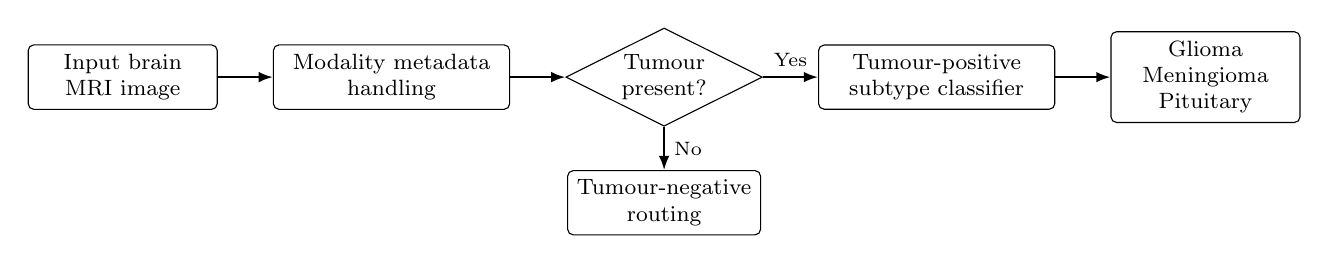
\begin{tikzpicture}[
node distance=0.55cm and 0.70cm,
box/.style={rectangle, rounded corners=2pt, draw, align=center, minimum width=2.4cm, minimum height=0.78cm, font=\footnotesize},
widebox/.style={rectangle, rounded corners=2pt, draw, align=center, minimum width=3.0cm, minimum height=0.78cm, font=\footnotesize},
decision/.style={diamond, aspect=2.0, draw, align=center, inner sep=1.2pt, font=\footnotesize},
arrow/.style={-{Latex[length=1.8mm]}, thick}
]
\node[box] (input) {Input brain\\MRI image};
\node[widebox, right=of input] (modality) {Modality metadata\\handling};
\node[decision, right=of modality] (binary) {Tumour\\present?};
\node[box, below=of binary] (negative) {Tumour-negative\\routing};
\node[widebox, right=of binary] (subtype) {Tumour-positive\\subtype classifier};
\node[box, right=of subtype] (classes) {Glioma\\Meningioma\\Pituitary};
\draw[arrow] (input) -- (modality);
\draw[arrow] (modality) -- (binary);
\draw[arrow] (binary) -- node[above, font=\scriptsize]{Yes} (subtype);
\draw[arrow] (binary) -- node[right, font=\scriptsize]{No} (negative);
\draw[arrow] (subtype) -- (classes);
\end{tikzpicture}
}
\caption{Hierarchical workflow for MRI input handling, tumour detection, and tumour subtype classification.}
\label{fig:hierarchical-workflow}
\end{figure}

\subsection{Datasets and Preprocessing}

For the binary brain tumour detection task, which classifies MRI images as tumour-positive or tumour-negative, two publicly available brain MRI datasets from Kaggle were combined. Dataset 1, Brain MRI Images for Brain Tumour Detection, was contributed by Navoneel Chakrabarty and contains 253 MRI images in total, with 155 tumour-positive and 98 tumour-negative images. These images represent a mixture of T1-weighted and T2-weighted sequences, although specific sequence information is not uniformly provided. Dataset 2, Brain Tumour Detection, was contributed by Ahmed Hamada and contains 3,000 MRI images, with a balanced distribution of 1,500 tumour-positive and 1,500 tumour-negative images. The combined binary dataset therefore contains 3,253 images, with 1,655 tumour-positive and 1,598 tumour-negative samples.

\begin{figure}[htbp]
\centering
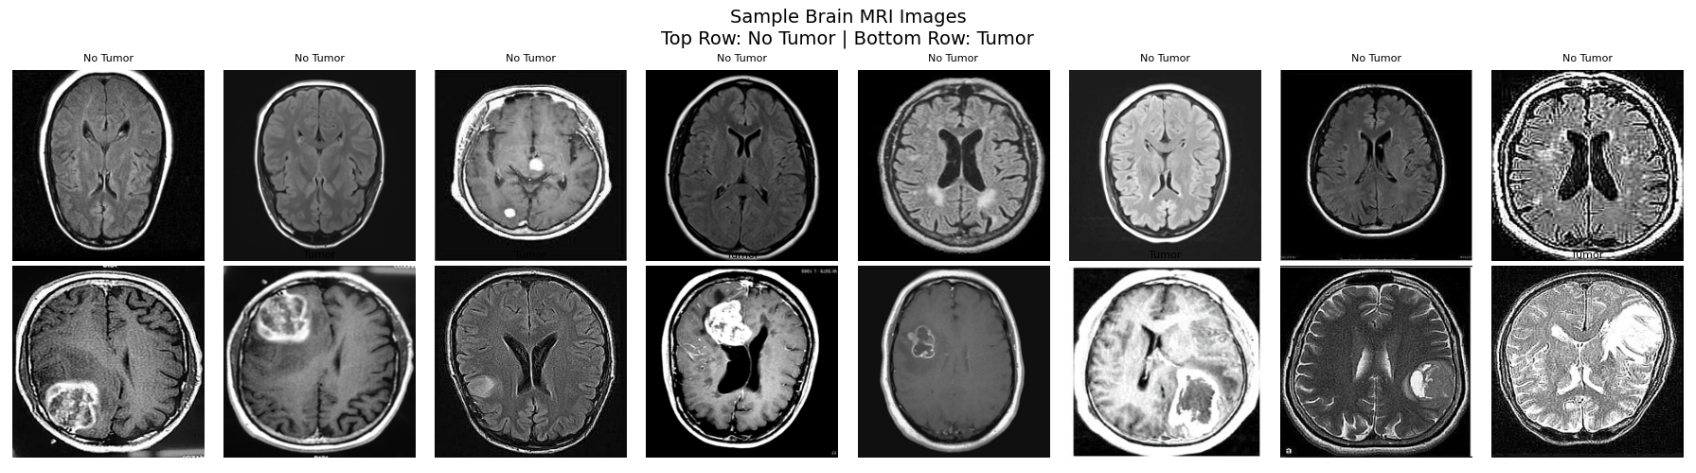
\includegraphics[width=\textwidth]{figures/detection_sample_brain_mri_images.png}
\caption{Representative brain MRI images used for binary tumour detection.}
\label{fig:representative-brain-mri-images-used-for-bina}
\end{figure}

The images are provided in JPEG format and have been pre-cropped to focus on the brain region, though some variability in field of view and image resolution exists across samples. The combined binary dataset therefore comprised 3,253 images, with 1,598 non-tumour images (49.1\%) and 1,655 tumour-positive images (50.9\%).

\begin{figure}[htbp]
\centering
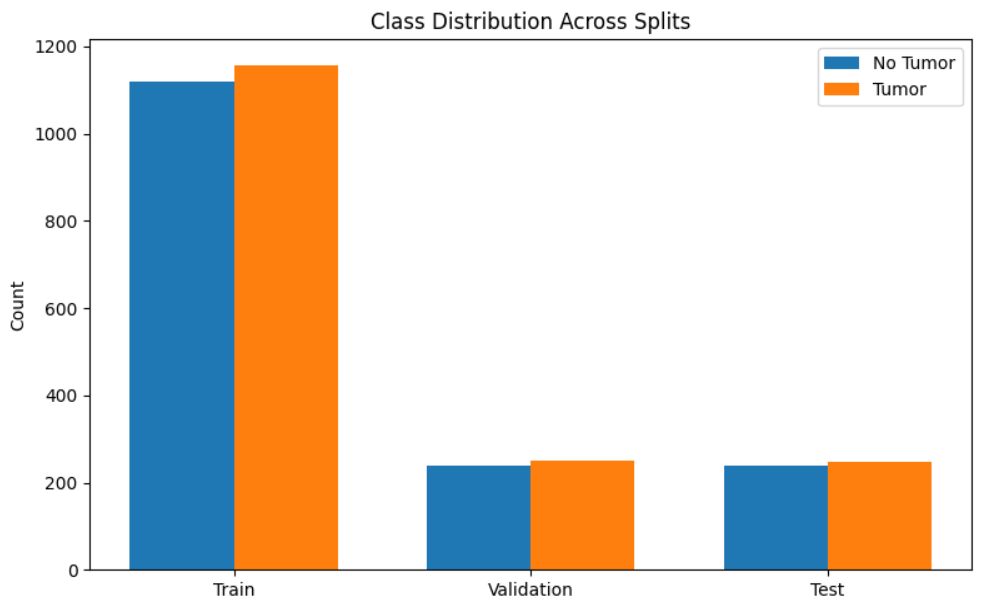
\includegraphics[width=\linewidth]{figures/detection_dataset_class_distribution.png}
\caption{Class distribution of the binary tumour detection dataset.}
\label{fig:class-distribution-of-the-binary-tumour-detec}
\end{figure}

This near-perfect balance prevents the model from exploiting class imbalance and ensures that chance-level accuracy remains at 50\%. For the more challenging multiclass classification task, where the model must distinguish between glioma, meningioma, and pituitary tumours, two publicly available brain tumour MRI datasets were combined. Dataset 1, Sartaj Bhuvaji's Brain Tumour Classification MRI, provides a structured collection with separate training and testing folders organised into three class subdirectories, with all images in JPEG format at a consistent $224\times 224$ pixels.

\begin{figure}[htbp]
\centering
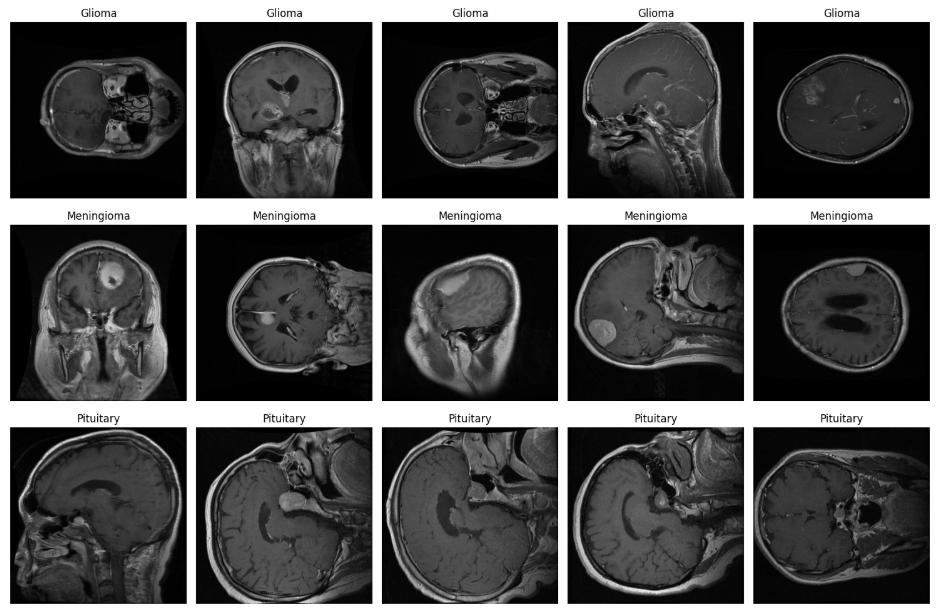
\includegraphics[width=0.88\textwidth]{figures/classification_sample_mri_by_tumour_type.png}
\caption{Representative MRI images for multiclass tumour classification.}
\label{fig:representative-mri-images-for-multiclass-tumo}
\end{figure}

Images of the brain tumours in question taken from the Jun Cheng's Brain Tumour MRI Dataset were in the form of JPEG. the merged multiclass dataset prior to deduplication consisted of 5,828 images; glioma being the largest subset at 40.4\%, making up 2,352 images, meningioma at 28.2\% and having 1,645 images, and pituitary making up for 31.4\% with 1,831 images.

\begin{figure}[htbp]
\centering
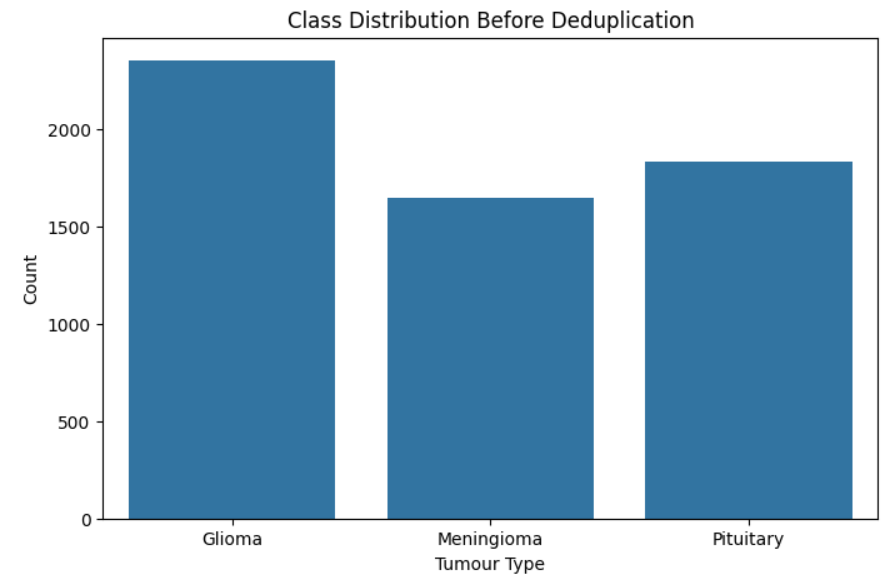
\includegraphics[width=\linewidth]{figures/classification_class_distribution_before_deduplication.png}
\caption{Class distribution before perceptual hash based deduplication.}
\label{fig:class-distribution-before-perceptual-hash-bas}
\end{figure}

Systematic deduplication was necessary for the multiclass dataset because images collected from multiple public sources may contain duplicate or near-duplicate versions of the same scan. Such images may differ only because of resizing, compression, contrast adjustment, or minor format conversion. If near-duplicates are distributed across training, validation, and test splits, the evaluation can be inflated because the model may recognise visual memory rather than learn a generalisable representation. To reduce this risk, perceptual hashing was applied before splitting. Each image was converted into a compact perceptual fingerprint using imagehash.phash, and pairs with Hamming distance less than or equal to 5 were treated as near-duplicates. This procedure reduced the multiclass dataset from 5,828 images to 4,705 unique images and protected the train-validation-test split from duplicate leakage.

Perceptual hashing was preferred over file-name matching and cryptographic hashing because the public MRI images may be visually identical even when their stored bytes differ. A scan can be resized, recompressed, renamed, or contrast-adjusted and still represent the same underlying visual evidence. Exact hashes such as MD5 or SHA-style hashes would treat such files as unrelated, whereas perceptual hashes encode the visual structure of the image. The Hamming tolerance of 5 gives the procedure a controlled margin for near-duplicate detection without treating genuinely different tumour appearances as duplicates. Applying this step before train-validation-test splitting is essential, because deduplicating after splitting would still allow leakage to influence the split composition.

\begin{figure}[htbp]
\centering
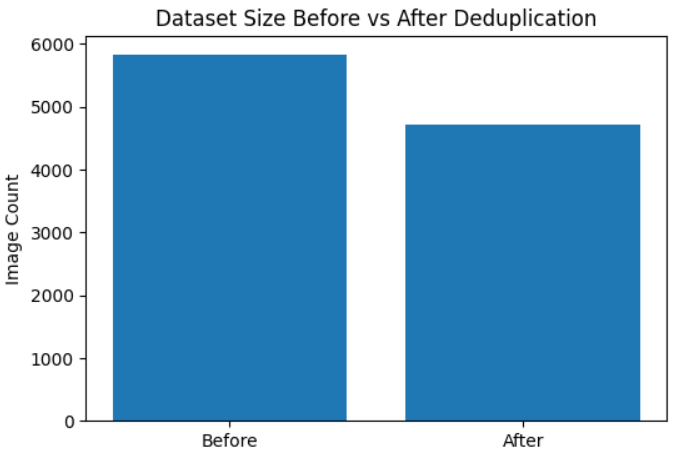
\includegraphics[width=\linewidth]{figures/classification_dataset_size_comparison_deduplication.png}
\caption{Dataset size before and after perceptual hash based deduplication.}
\label{fig:dataset-size-before-and-after-perceptual-hash}
\end{figure}

The final class distribution was glioma 2,000 (42.5\%), meningioma 1,304 (27.7\%), and pituitary 1,401 (29.8\%).

\begin{figure}[htbp]
\centering
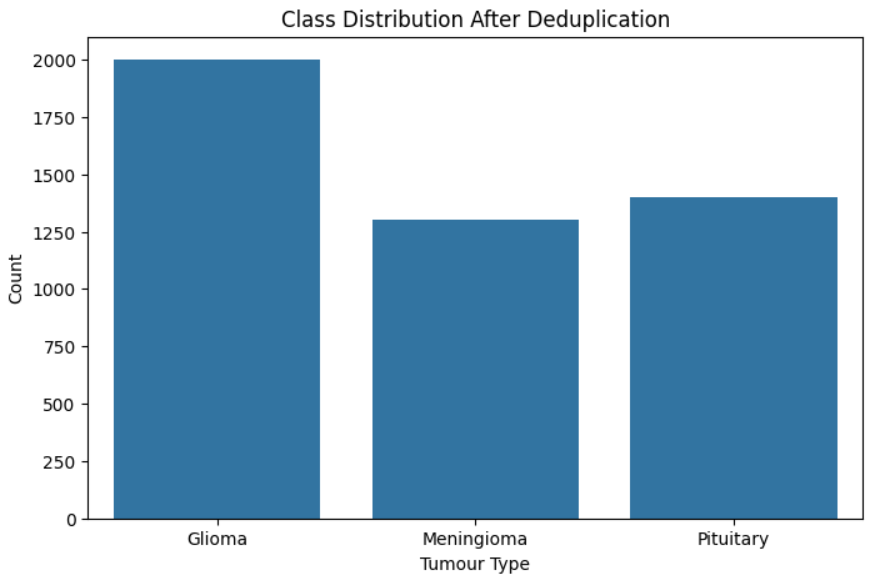
\includegraphics[width=\linewidth]{figures/classification_class_distribution_after_deduplication.png}
\caption{Class distribution after perceptual hash based deduplication.}
\label{fig:class-distribution-after-perceptual-hash-base}
\end{figure}

Stratification was employed for both splits in order to ensure that all of the samples had a representative distribution of the classes. In the case of binary detection, 3,253 images were divided up into 70\%/15\%/15\% training/validation/testing splits, which resulted in datasets consisting of 2,277, 488, and 488 images, respectively. With regard to multiclass classification, the same 70\%/15\%/15\% proportions were utilised for splitting 4,705 deduplicated images, which resulted in 3,293 training, 706 validation, and 706 testing images.

\begin{figure}[htbp]
\centering
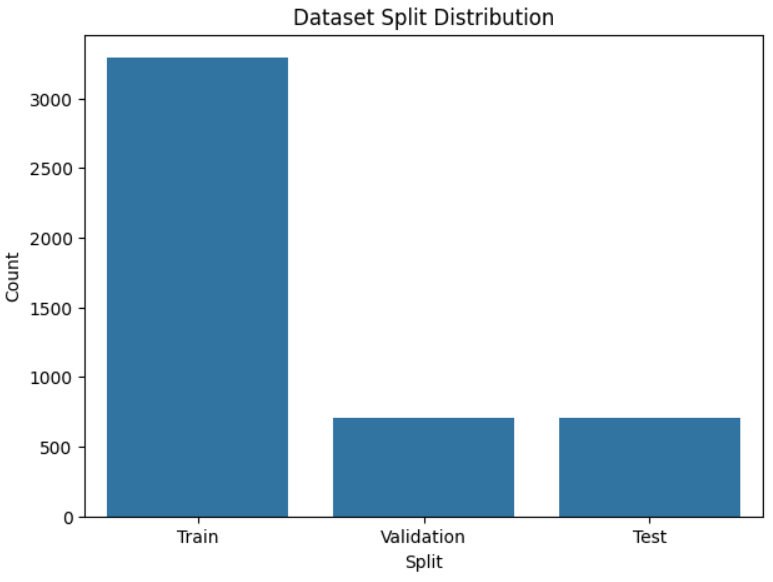
\includegraphics[width=\linewidth]{figures/classification_dataset_split_distribution.png}
\caption{Train, validation, and test split distribution for the deduplicated multiclass dataset.}
\label{fig:train-validation-and-test-split-distribution-}
\end{figure}

All images were converted to RGB format to maintain compatibility with ImageNet pretrained backbones. Images were resized to model-specific input dimensions: 224 by 224 pixels for ResNet50, VGG16, DenseNet121, EfficientNetB0, MobileNetV3-Large, ViT-B/16, Swin Transformer Base, and CoaTNet-0, and 299 by 299 pixels for InceptionV3. ImageNet normalisation statistics were applied using mean values of [0.485, 0.456, 0.406] and standard deviations of [0.229, 0.224, 0.225]. To improve generalisation, augmentation was applied only to the training set: random horizontal flipping with probability 0.5, random rotation up to 10 degrees, and colour jitter for brightness and contrast up to 20\%. Validation and test images used only deterministic resizing and normalisation.

\begin{figure}[htbp]
\centering
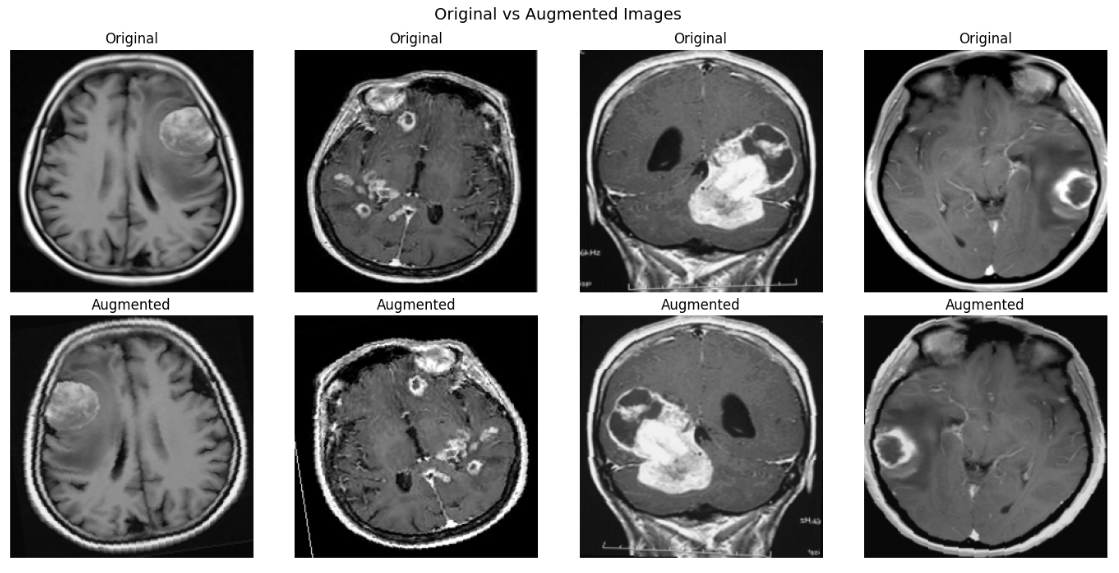
\includegraphics[width=0.90\textwidth]{figures/detection_mri_image_augmentation_comparison.png}
\caption{Augmentation examples used for binary tumour detection training.}
\label{fig:augmentation-examples-used-for-binary-tumour-}
\end{figure}

\begin{figure}[htbp]
\centering
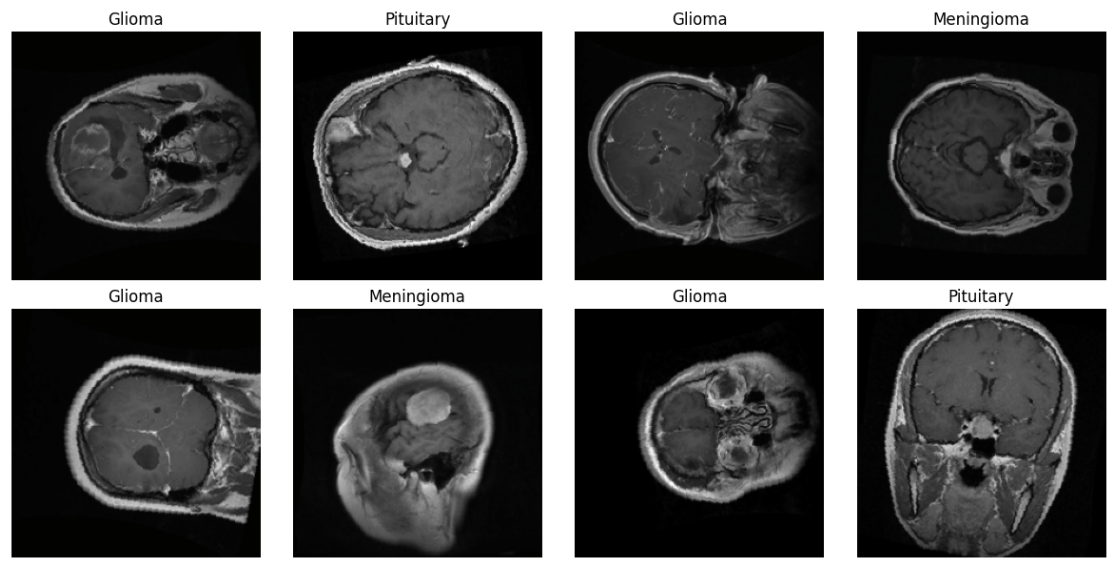
\includegraphics[width=0.90\textwidth]{figures/classification_augmented_mri_samples.png}
\caption{Augmentation examples used for multiclass tumour classification training.}
\label{fig:augmentation-examples-used-for-multiclass-tum}
\end{figure}

For validation and testing, only the essential transformations of resizing, tensor conversion, and normalisation were applied, with no stochastic augmentations, ensuring deterministic and reproducible evaluation.

The PyTorch DataLoader was configured with multi-GPU training optimisations: the number of worker subprocesses was set to 4, pin memory was enabled for faster CPU-to-GPU transfer, persistent workers were used to maintain worker processes across epochs, and a prefetch factor of 4 was set to hide data loading latency.

ResNet50 is a 50-layer residual network built around bottleneck residual blocks with skip connections that address the vanishing gradient problem. It contains 25.6 million parameters and was pre-trained on ImageNet. The final fully connected layer was replaced with a linear layer for binary (1 output) or multiclass (3 outputs) classification. VGG16 is a 16-layer network using only $3\times 3$ convolutional filters stacked in increasing depth, with 138 million parameters. Its classifier head was replaced appropriately for each task. DenseNet121 is a 121-layer densely connected network that concatenates feature maps of all preceding layers, maximising information flow with only 8 million parameters. The final classifier layer was modified for each task. EfficientNetB0, developed through neural architecture search and compound scaling, achieves state-of-the-art accuracy with only 5.3 million parameters. MobileNetV3-Large uses depth-wise separable convolutions for mobile and embedded applications, containing 5.4 million parameters. InceptionV3 is a 48-layer network with parallel convolutional paths of different kernel sizes ($1\times 1$, $3\times 3$, $5\times 5$) within inception modules, capturing multi-scale features with 23.9 million parameters. ViT-B/16 divides the input image into $16\times 16$ patches, processing them as a sequence with a transformer encoder, containing 86 million parameters and lacking inherent convolutional inductive biases. Swin Transformer Base introduces hierarchical transformers with shifted windows, achieving linear complexity and multi-scale processing with 88 million parameters. CoaTNet-0 combines convolutional and attention mechanisms in a unified architecture with approximately 10 million parameters.

All experiments were conducted on dual NVIDIA Tesla T4 GPUs with 16 GB GDDR6 memory each, Intel Xeon processors with 4 virtual CPUs, and 29 GB of RAM. The software environment included Python 3.12.12, PyTorch 2.x with CUDA 12.x, Torchvision, the TIMM library for transformer architectures, TensorBoard for tracking, and scikit-learn for metrics. Multi-GPU training used torch.nn.DataParallel, and mixed precision training with FP16 was employed via torch.amp.autocast and GradScaler. To ensure fair comparison, the following hyperparameters were standardised across all models: 10 epochs of training, AdamW optimiser with weight decay 0.01, learning rate $3 \times 10^{-4}$, CosineAnnealingLR scheduler with T\_max=10, BCEWithLogitsLoss for binary classification and CrossEntropyLoss for multiclass, and model-specific batch sizes (ResNet50: 256, VGG16: 256, DenseNet121: 64, EfficientNetB0: 256, MobileNetV3-Large: 256, InceptionV3: 128, ViT-B/16: 128, Swin Base: 64, CoaTNet-0: 64) set to the maximum that fit within GPU memory. The training loop for each epoch consisted of a training phase with augmentations and weight updates, and a validation phase without augmentations or gradient computation. Learning rate scheduling was applied after each epoch, and model checkpointing saved the best model based on validation AUC for binary detection or validation accuracy for multiclass classification. The run\_epoch function handled both modes with a unified code path, using autocast, gradient scaling, and accumulation of predictions for metric computation.

The evaluation metrics were accuracy, cross-entropy loss, and AUC-ROC. Accuracy provides an intuitive measure of the proportion of correctly classified images, while loss captures calibration and prediction confidence. AUC-ROC was included because it measures the ranking ability of the model across thresholds, ranging from 0.5 for random discrimination to 1.0 for perfect separation. For multiclass classification, a one-versus-rest formulation was applied to compute AUC for each class and the aggregate score. Random seed control was implemented with SEED=42 for PyTorch, NumPy, and Python modules. CUDA deterministic settings were used where practical, while cudnn.benchmark remained enabled for speed. The complete working code is publicly available through the repository listed in Appendix C.

\section{Results and Discussion}

The InceptionV3 model delivered 99.39\% accuracy with an ideal AUC score of 1.0000. Its convergence behaviour was also strong: after the first epoch, training accuracy had already reached 89.80\% with validation AUC of 0.9997, and by the second epoch, training accuracy increased to 99.22\% with validation AUC of 0.9999. CoaTNet-0 began with lower first-epoch training accuracy and AUC values of 65.27\% and 0.8437, respectively, but continued improving until the seventh epoch and ultimately reached the best binary detection accuracy of 99.59\%. EfficientNetB0 matched this accuracy with far fewer parameters, demonstrating that compound-scaled CNNs are highly suitable for this dataset. Swin Base reached 98.16\% accuracy with AUC of 0.9990, requiring more epochs to converge from 61.25\% training accuracy and AUC 0.7959 at epoch 1 to best validation performance at epoch 6. MobileNetV3 exhibited training instability with a large gap between training and validation behaviour; the best validation AUC of 0.9993 was achieved at epoch 10 despite 99.90\% training accuracy, but test accuracy dropped to 91.39\%, indicating weak generalisation. ViT-B/16 showed the slowest convergence and reached its best validation only at epoch 10, with final test accuracy of 95.08\% and AUC of 0.9861. VGG16 performed worst, with final test accuracy of only 83.20\% and AUC of 0.9247, indicating that this classical high-parameter architecture is not suitable for the present medical imaging setting without stronger regularisation or additional data.

\begin{figure}[htbp]
\centering
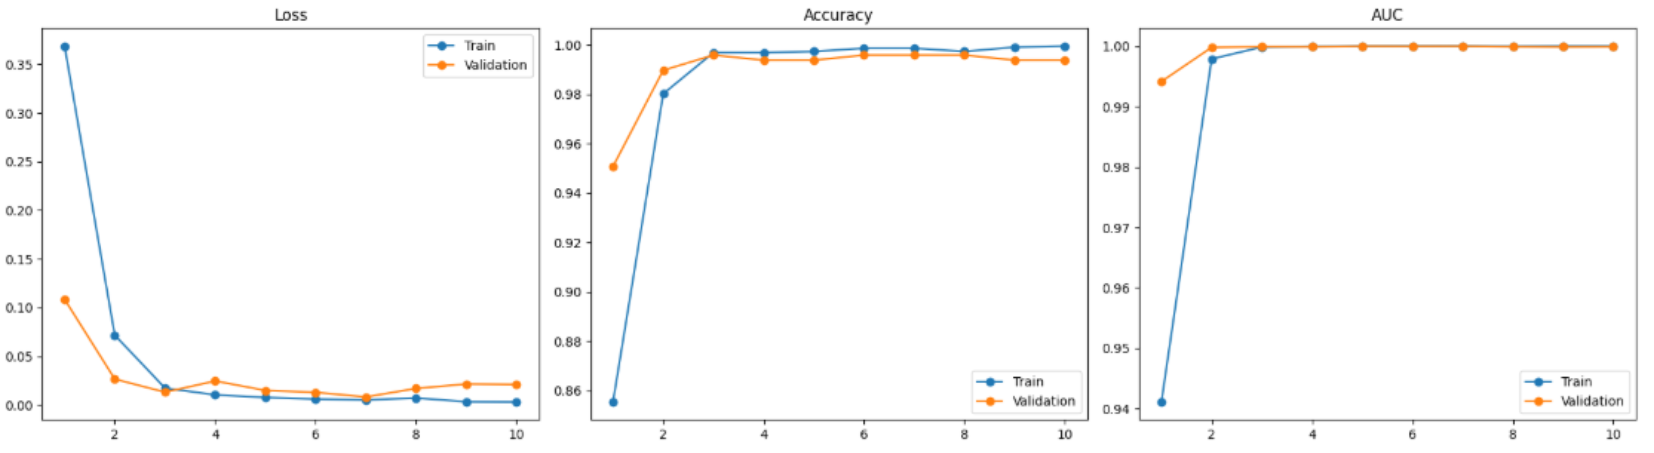
\includegraphics[width=\textwidth]{figures/detection_model_training_metrics_curves.png}
\caption{Training and validation metric curves for binary tumour detection.}
\label{fig:training-and-validation-metric-curves-for-bin}
\end{figure}

\begin{table}[htbp]
\centering
\caption{Binary Detection Test Results}
\label{tab:binary-test-results}
\scriptsize
\begin{tabular*}{\textwidth}{@{\extracolsep{\fill}}lcccc@{}}
\toprule
Model & Test Acc. & Test AUC & Best Val. AUC & Params \\
\midrule
InceptionV3 & 99.39\% & 1.0000 & 0.9999 (Epoch 2) & 23.9M \\
CoaTNet-0 & 99.59\% & 1.0000 & 0.9999 (Epoch 7) & \textasciitilde{}10M \\
EfficientNetB0 & 99.59\% & 0.9999 & 0.9999 (Epoch 4) & 5.3M \\
DenseNet121 & 97.95\% & 0.9999 & 1.0000 (Epoch 1) & 8.0M \\
ResNet50 & 99.39\% & 0.9999 & 0.9999 (Epoch 6) & 25.6M \\
Swin Base & 98.16\% & 0.9990 & 0.9988 (Epoch 6) & 88M \\
MobileNetV3 & 91.39\% & 0.9982 & 0.9993 (Epoch 10) & 5.4M \\
ViT-B/16 & 95.08\% & 0.9861 & 0.9897 (Epoch 10) & 86M \\
VGG16 & 83.20\% & 0.9247 & 0.9343 (Epoch 10) & 138M \\
\bottomrule
\end{tabular*}
\end{table}

\begin{figure}[htbp]
\centering
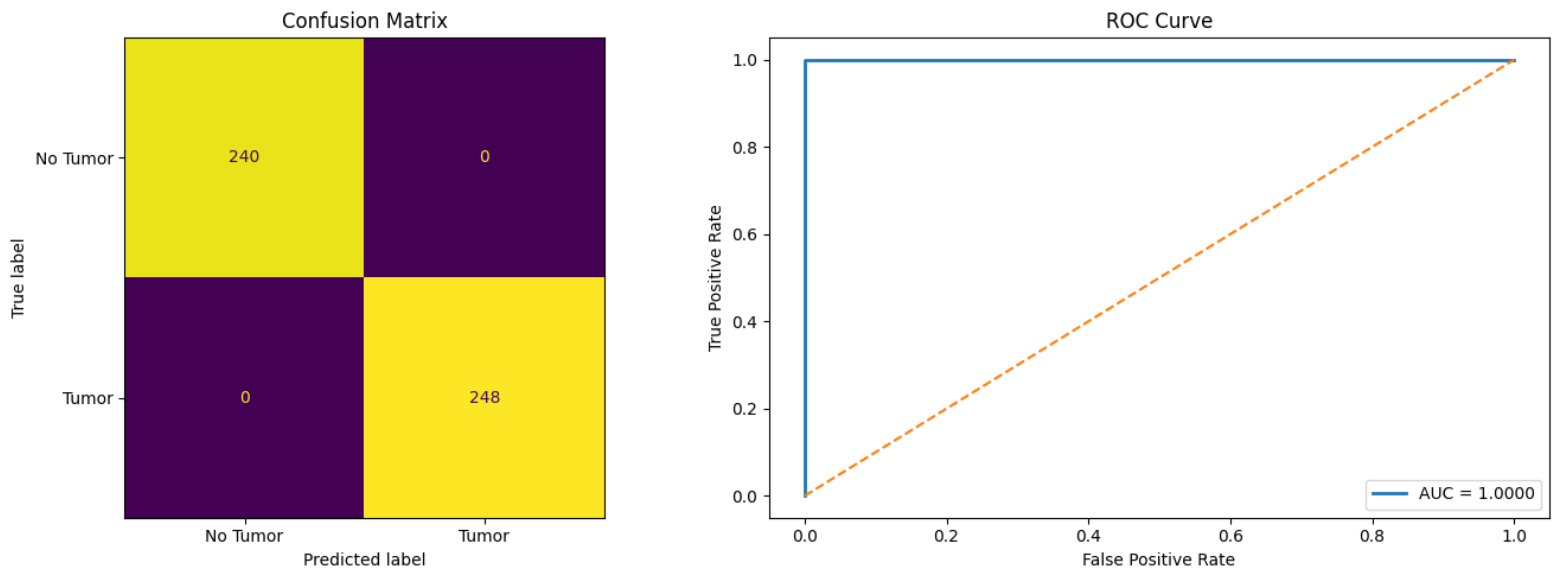
\includegraphics[width=0.95\textwidth]{figures/detection_confusion_matrix_roc_curve.png}
\caption{Confusion matrix and ROC curve for binary tumour detection.}
\label{fig:confusion-matrix-and-roc-curve-for-binary-tum}
\end{figure}

The findings of the multiclass brain tumour classification experiment are displayed in Table~\ref{tab:multiclass-test-results}. Both InceptionV3 and Swin Base performed equally well in terms of accuracy at 98.58\%. InceptionV3 was very efficient, reaching 99.88\% accuracy after epoch 10. Similarly, Swin Base was able to reach the same level of accuracy in an equal number of epochs. However, in terms of test loss, Swin Base had the least at 0.0377. Whereas EfficientNetB0 and CoaTNet-0 achieved equal accuracy levels of 97.59\%. EfficientNetB0 had the highest accuracy to parameter ratio, with 5.3 million parameters. On the contrary, ViT-B/16 underperformed with an accuracy level of only 89.52\%. With 4,705 images available, the transformers were unable to learn effectively.

\begin{figure}[htbp]
\centering
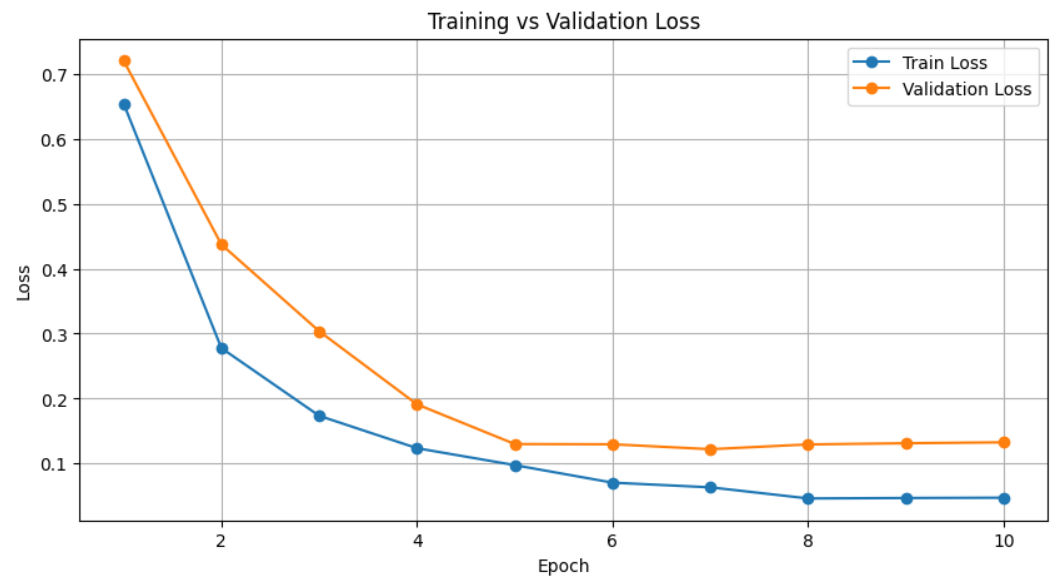
\includegraphics[width=\linewidth]{figures/classification_training_vs_validation_loss_curves.png}
\caption{Training and validation loss curves for multiclass tumour classification.}
\label{fig:training-and-validation-loss-curves-for-multi}
\end{figure}

\begin{figure}[htbp]
\centering
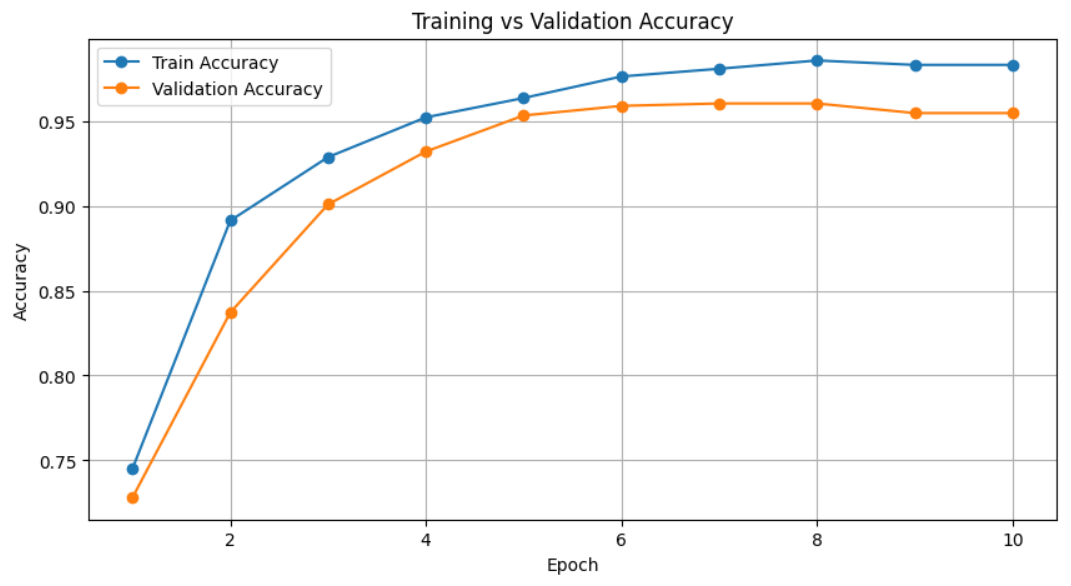
\includegraphics[width=\linewidth]{figures/classification_training_vs_validation_accuracy.png}
\caption{Training and validation accuracy curves for multiclass tumour classification.}
\label{fig:training-and-validation-accuracy-curves-for-m}
\end{figure}

\begin{figure}[htbp]
\centering
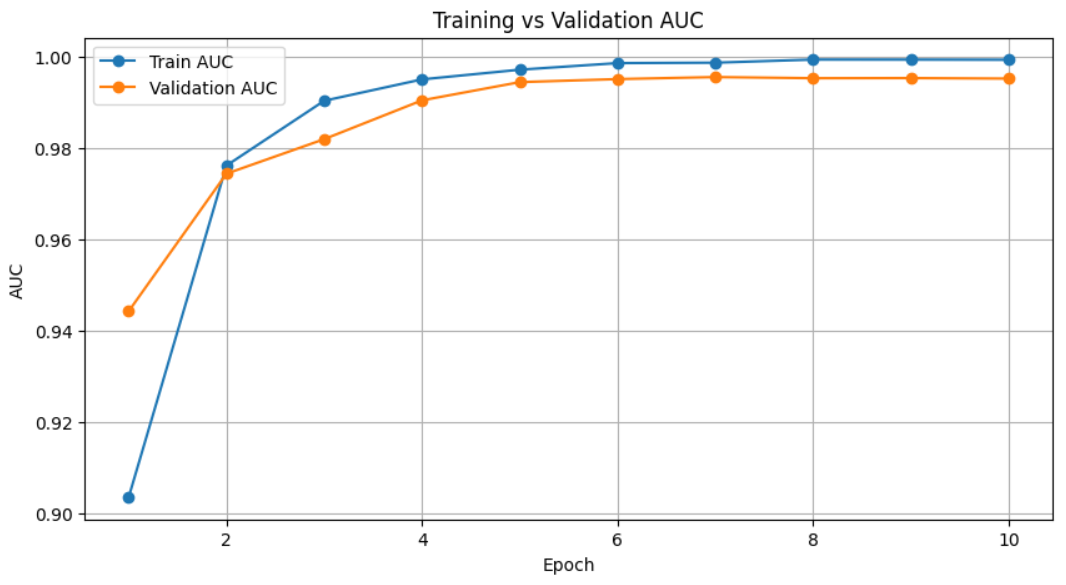
\includegraphics[width=\linewidth]{figures/classification_training_vs_validation_auc_curves.png}
\caption{Training and validation AUC curves for multiclass tumour classification.}
\label{fig:training-and-validation-auc-curves-for-multic}
\end{figure}

\begin{table}[htbp]
\centering
\caption{Multiclass Classification Test Results}
\label{tab:multiclass-test-results}
\scriptsize
\begin{tabular*}{\textwidth}{@{\extracolsep{\fill}}lcccc@{}}
\toprule
Model & Test Acc. & Test Loss & Test AUC & Params \\
\midrule
InceptionV3 & 98.58\% & 0.0389 & 0.9995 & 27.2M \\
Swin Base & 98.58\% & 0.0377 & 0.9993 & 86.7M \\
EfficientNetB0 & 97.59\% & 0.0582 & 0.9987 & 5.3M \\
CoaTNet-0 & 97.59\% & 0.0638 & 0.9990 & \textasciitilde{}10M \\
ResNet50 & 96.60\% & 0.0740 & 0.9990 & 25.6M \\
ViT-B/16 & 89.52\% & 0.2737 & 0.9736 & 86.4M \\
\bottomrule
\end{tabular*}
\end{table}

\begin{figure}[htbp]
\centering
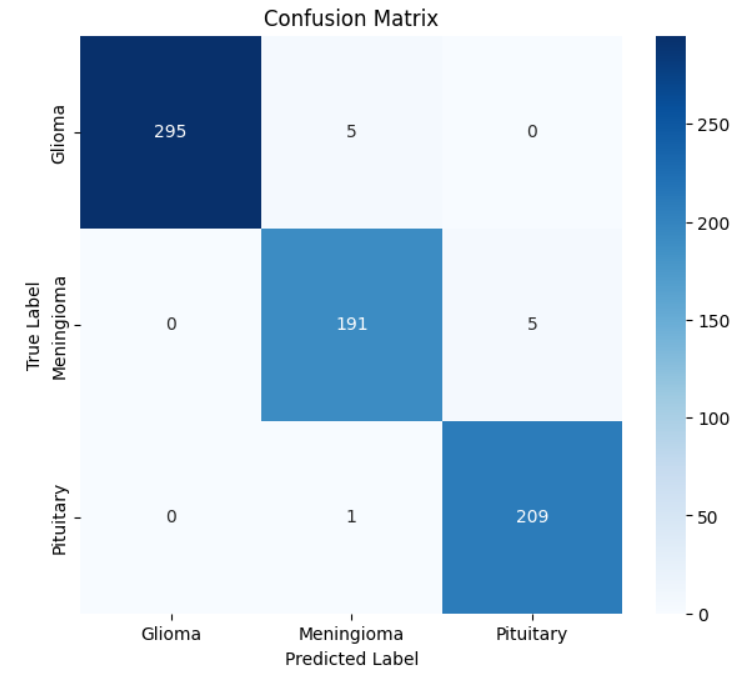
\includegraphics[width=0.95\linewidth]{figures/classification_tumour_classification_confusion_matrix.png}
\caption{Confusion matrix for multiclass tumour classification.}
\label{fig:confusion-matrix-for-multiclass-tumour-classi}
\end{figure}

\begin{figure}[htbp]
\centering
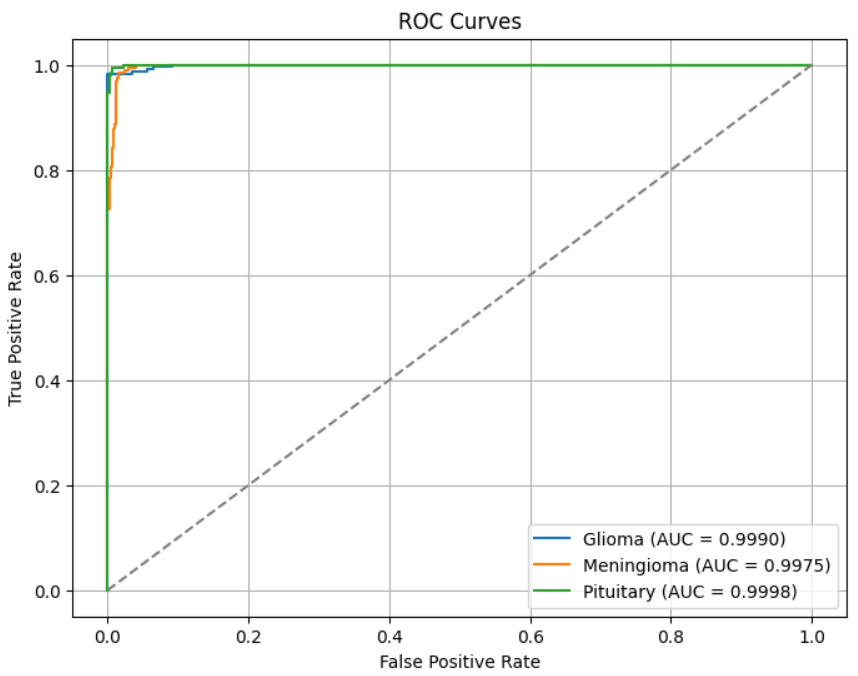
\includegraphics[width=0.95\linewidth]{figures/classification_multiclass_roc_curves.png}
\caption{One versus rest ROC curves for multiclass tumour classification.}
\label{fig:one-versus-rest-roc-curves-for-multiclass-tum}
\end{figure}

Table~\ref{tab:model-efficiency} presents the computational efficiency comparison. EfficientNetB0 was the fastest and most memory-efficient model, enabling batch size 256. InceptionV3 offered an excellent balance of high accuracy and moderate computational cost. Swin Base and ViT-B/16 required significantly more training time and memory due to their self-attention mechanisms. The accuracy per million parameters metric highlights architectural efficiency: EfficientNetB0 achieved 0.188\% per million parameters, DenseNet121 0.122\%, CoaTNet-0 approximately 0.0996\%, InceptionV3 0.0416\%, ResNet50 0.0388\%, Swin Base 0.0112\%, ViT-B/16 0.0111\%, and VGG16 only 0.0060\%.

\begin{table}[htbp]
\centering
\caption{Model Efficiency Comparison}
\label{tab:model-efficiency}
\scriptsize
\begin{tabular*}{\textwidth}{@{\extracolsep{\fill}}lcccc@{}}
\toprule
Model & Batch & Params & Rel. Speed & Memory \\
\midrule
EfficientNetB0 & 256 & 5.3M & 1.0x (Fastest) & Lowest \\
ResNet50 & 256 & 25.6M & 1.2x & Low \\
CoaTNet-0 & 64 & \textasciitilde{}10M & 2.5x & Moderate \\
InceptionV3 & 128 & 23.9--27.2M & 2.0x & Moderate \\
Swin Base & 64 & 86--88M & 4.0x & High \\
ViT-B/16 & 32 & 86--86.4M & 5.0x & Highest \\
VGG16 & 256 & 138M & 1.5x & Moderate \\
\bottomrule
\end{tabular*}
\end{table}

Table~\ref{tab:comparison-literature} compares the present results with previously published studies. The ResNet50 and InceptionV3 results align with or exceed the earlier benchmarks, which supports the effectiveness of the standardised training pipeline. The large gap for VGG16, where the present test accuracy is 83.20\% compared with the reported 98.69\%, is likely related to differences in preprocessing, augmentation, train-test splitting, and duplicate handling. The DenseNet121 result of 97.95\% is slightly below the reported 99.51\%, suggesting that the combined and deduplicated dataset is more difficult than single-source evaluations. These differences also show why direct comparison between papers is fragile when dataset construction and duplicate control are not described in detail.

\begin{table}[htbp]
\centering
\caption{Comparison With Existing Literature}
\label{tab:comparison-literature}
\scriptsize
\begin{tabularx}{\textwidth}{@{}YYcccc@{}}
\toprule
Study & Model & Dataset Size & Task & Reported Accuracy & This Study Result \\
\midrule
Talo et al. (2019) \cite{ref16} & ResNet50 & 253 & Binary & 95.23\% & 99.39\% \\
Khan et al. (2020) \cite{ref23} & VGG16 & 3,064 & Binary & 98.69\% & 83.20\% \\
Noreen et al. (2020) \cite{ref24} & DenseNet121 & 3,064 & Binary & 99.51\% & 97.95\% \\
Rehman et al. (2020) \cite{ref25} & InceptionV3 & 3,064 & Binary & 99.34\% & 99.39\% \\
Deepak and Ameer (2019) \cite{ref15} & InceptionV3 & 3,064 & Multiclass & 97.50\% & 98.58\% \\
\bottomrule
\end{tabularx}
\end{table}

Several architectural innovations explain the observed performance patterns in medical imaging tasks. Residual learning in ResNet and EfficientNet supports deeper feature extraction, while dense connections in DenseNet maximise feature reuse with fewer parameters. Inception modules capture tumour appearances at multiple spatial scales through parallel convolutional paths. Attention mechanisms in CoaTNet and Swin Transformer model longer-range contextual relationships between tumour regions and surrounding healthy tissue. Neural architecture search in EfficientNet and MobileNetV3 improves the balance between accuracy and parameter efficiency. The results also illustrate a transformer paradox: the pure ViT model underperformed, while the hybrid CoaTNet model performed strongly. This suggests that transformer-only architectures may require more data than the available 3,253 to 4,705 images to reach their full potential in this setting.

The binary and multiclass experiments also show that high AUC values should be interpreted together with accuracy, loss, and efficiency. Several binary models reached AUC values close to 1.0000, but their test accuracies and generalisation patterns were not identical. MobileNetV3, for example, achieved a strong validation AUC while showing lower final test accuracy, indicating that ranking performance alone may hide threshold-level weaknesses. Similarly, VGG16 has a very large parameter count but did not generalise well under the present settings. In contrast, EfficientNetB0 maintained strong accuracy with a small parameter footprint, making it a better candidate for constrained deployment. These observations support the view that model choice in medical imaging should not be based only on the highest single metric. A clinically useful model should combine accuracy, stability, calibration, low false-negative risk, reproducibility, and feasible inference cost.

The deduplicated multiclass experiment is particularly important for interpreting the subtype results. Public brain MRI classification datasets often circulate through multiple mirrors, converted formats, and reorganised folder structures. Without near-duplicate filtering, the same or visually equivalent image can appear in both training and testing subsets, causing the measured performance to reflect memorisation. The use of perceptual hash filtering before splitting makes the reported multiclass results more conservative and more credible. The reduction from 5,828 to 4,705 images also explains why the multiclass task is harder than it may appear from raw dataset size alone. The final dataset remains large enough for transfer learning, but the removal of repeated visual evidence creates a stronger test of generalisation across glioma, meningioma, and pituitary tumour appearances.

\subsection{Deployment Recommendations}

The recommended model depends on the intended deployment context. For cloud-based or high-accuracy diagnostic support, InceptionV3 is a strong choice because it achieved near-perfect binary detection performance with moderate computational requirements. For edge devices and resource-constrained hospitals, EfficientNetB0 is the preferred model because it achieved 99.59\% binary detection accuracy with only 5.3 million parameters and also remained highly competitive in multiclass classification. MobileNetV3 may be considered for mobile applications where memory is limited, although its generalisation was weaker than EfficientNetB0. ResNet50 remains a useful research baseline because it is widely understood and reproducible. No single architecture is universally optimal; model selection should balance accuracy, inference cost, memory footprint, and the clinical setting in which the tool will be used.

In a hospital workflow, the most practical use of the system would be triage and second-reader support rather than autonomous diagnosis. A tumour-negative binary output could help prioritise routine cases, while tumour-positive outputs could be flagged for radiologist review and then routed to the subtype classifier for glioma, meningioma, or pituitary prediction. This staged approach is especially relevant in settings where neuroradiology expertise is limited and MRI reporting queues are long. However, each prediction should be displayed with confidence information, and uncertain cases should be escalated rather than silently accepted. The model should also be evaluated on external hospital images before deployment because public Kaggle datasets may not represent scanner variation, acquisition protocols, demographic diversity, image artefacts, or postoperative and treatment-related changes. For district hospitals and low-resource centres, EfficientNetB0 offers the best balance of accuracy and computational cost. For tertiary centres with stronger infrastructure, InceptionV3 or CoaTNet-0 may be preferred when marginal accuracy improvements are more important than inference efficiency.

\begin{figure}[htbp]
\centering
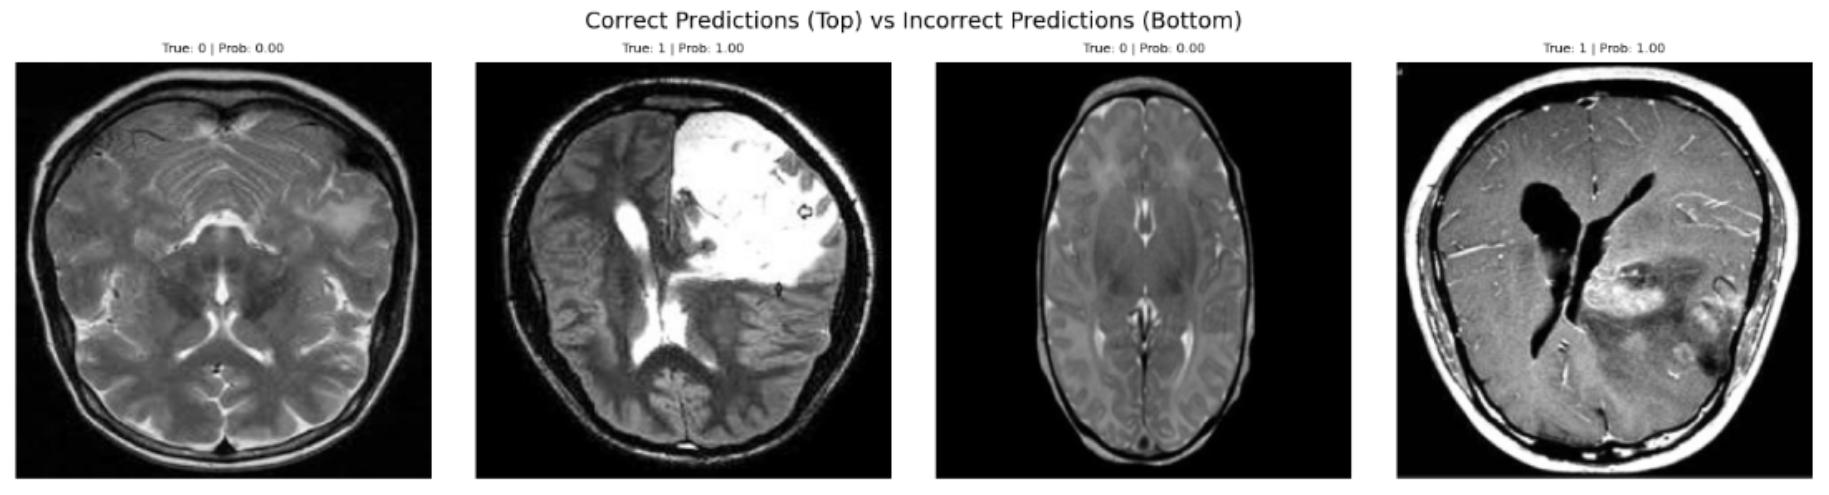
\includegraphics[width=\textwidth]{figures/detection_model_prediction_examples.png}
\caption{Representative binary tumour detection predictions.}
\label{fig:representative-binary-tumour-detection-predic}
\end{figure}

\section{Limitations and Future Work}

The sample size between 3,253 and 4,705 is relatively small and may not represent clinical heterogeneity for diverse patient cohorts, MRI protocols, field strength, and scanner brands. There is an availability of limited samples from two or three publicly available datasets, which may be lacking in terms of geographic and demographic diversity. The annotation of the data involves binary or trinary classes, but there is a lack of grade, exact localisation, and size information for each instance. There could also be some noise in the labels for crowdsourced datasets. Since the models have been trained using the Kaggle dataset, they may not generalise to other hospitals' MRI protocols, and there was no external validation. Training of models has been restricted to ten epochs due to budget limitations, and most of the models converge in this range. However, there has been no hyper-parameter tuning per model, and only one training cycle has been conducted without cross-validation or ensembling. The main criteria for evaluating the models include accuracy, loss, and area under the curve (AUC). Model input consists of a single 2D slice as opposed to 3D volumes of MRI scans, thus neglecting the volume aspect, and support for multimodal MRI scans is also absent. Integration into clinical workflows and adherence to DICOM standards have not been considered, nor has inference time been measured.

Another limitation is that the datasets provide image-level labels rather than detailed radiological annotations. The binary detector learns whether an image is labelled tumour-positive or tumour-negative, but it does not learn tumour boundary, tumour size, oedema extent, mass effect, grade, molecular subtype, or treatment status. The multiclass classifier predicts glioma, meningioma, or pituitary tumour, but it does not distinguish tumour grade or clinically important subtypes within those categories. The two-dimensional slice format also means that inter-slice continuity and volumetric tumour context are not captured. These constraints do not invalidate the classification benchmark, but they define its intended use: preliminary image-level decision support rather than complete radiological reporting.

The results should also be interpreted as dataset-specific benchmark results rather than universal clinical performance estimates. Public MRI repositories are valuable for reproducible research, but they cannot fully represent scanner calibration, acquisition artefacts, referral bias, postoperative anatomy, motion degradation, or rare tumour appearances encountered in routine clinical practice. External validation is therefore necessary before any clinical claim is made in future clinical deployment studies.

Future improvements should focus on dataset extension by gathering more public datasets (BRATS, TCGA, institutional data), use of 5-fold cross-validation, and introduction of fine granularity of classifications for tumour type and grade. Future aspirations include cooperation with clinical institutions to gather diverse clinically approved data, construction of 3D models to enable volume segmentation using MRI images, and consideration of multi-sequence MRI input data. As for model improvements, one could try out different model architectures such as EfficientNetB7, Swin Large, ViT-Large, try to utilise ensemble learning for merging the best performing models, and try new architectures like ConvNeXt, MLP-Mixer, and FocalNet. For better training of models, one could consider extended training with early stopping, learning rate warm-up with cosine annealing with restarts, progressive resizing of images, and advanced image augmentation techniques like MixUp, CutMix, and RandAugment. Deployment tests should use external test datasets. Their assessment should be based on performance on lower quality images and by measuring the time taken for inference using edge devices. Then create DICOM-compliant inference pipelines with user interfaces and uncertainty estimation. Extended experiments should also investigate ablation studies on data augmentation, pre-training vs. training from scratch, batch size and learning rate experiments, and additional metrics such as precision, recall, F1 score, and inference time.

\section{Ethical Implications}

The main positive effect of this type of AI system is improved access to brain tumour screening in underserved areas. Additional benefits include reduced radiologist workload, greater consistency in preliminary assessment, and quicker triage in emergencies. Potential risks include overdependence on automated systems, unequal access to the technology, false negatives, and demographic or institutional bias in training data. MRI protocols may differ across hospitals, and tumour appearance may vary across population groups and scanner settings. Mitigation strategies include diverse data collection, subgroup performance analysis, transparent reporting of limitations, and human-in-the-loop review of every prediction. Pre-deployment requirements include regulatory approval such as FDA, CE Mark, or CDSCO clearance in India, multicentre validation, specification of operating thresholds, and user training. Organisational requirements include confidence thresholds for referral, performance tracking, incident reporting, and model update protocols. Transparency requirements include public disclosure of dataset sources, publication of validation studies, communication of model limitations to clinical users, and explainable artificial intelligence capabilities. In India, the Central Drugs Standard Control Organization oversees medical software applications under the Medical Devices Rules, 2017, and quality management system requirements such as ISO 13485 should be satisfied along with data privacy requirements under the Digital Personal Data Protection Act, 2023.

\section{Conclusion}

The current investigation is a thorough assessment of nine deep learning models for brain tumour analysis in comparable settings, contributing several practical findings. First, a standardised benchmark was introduced across CNNs, efficient CNNs, and transformer-based models using comparable image datasets, identical preprocessing strategies, and controlled hyperparameter settings. This addresses the missing-benchmark problem that often prevents fair inter-study comparison. Second, perceptual hash based deduplication eliminated 19.3\% of near-identical multiclass images, reducing the risk of data leakage and improving confidence in the reported generalisation results. Third, multi-architecture assessment was carried out across three model groups: classical CNNs, efficient CNNs, and transformer or hybrid transformer architectures. Fourth, performance was quantified through accuracy, loss, and AUC for both binary and multiclass tasks, providing a practical basis for model selection. Fifth, architecture-level features that contribute to improved performance were identified, including residual connections, dense feature reuse, multi-scale convolution, attention, and compound scaling. Sixth, recommendations were provided for practical implementation across cloud, edge, and research settings by balancing the accuracy-efficiency trade-off. Seventh, the accompanying code supports reproduction and further development of the results.

Performance levels for binary classification were at their highest for CoaTNet-0, EfficientNetB0, InceptionV3, and ResNet50 (above 99\% accuracy). Swin Base, DenseNet121, and ViT-B/16 performed well (accuracy ranging between 95 and 98\%). MobileNetV3 was sufficient (accuracy ranging between 90 and 95\%), while VGG16 was insufficient (below 90\% accuracy). The best performers in multiclass classification were InceptionV3 and Swin Base with a score of 98.58\%, followed by EfficientNetB0 and CoaTNet-0 (97.59\%) and ResNet50 (96.60\%). Finally, the ViT-B/16 had an accuracy rate of 89.52\%. The following key findings can be drawn from this analysis: contemporary architectures consistently outperform traditional architectures; the relationship between parameter efficiency and generalisation ability is evident, with EfficientNetB0 combining high accuracy with only 5.3 million parameters.

With the high level of accuracy rates recorded (greater than 99\% for binary detection and greater than 98\% for multiclass classification), automated deep learning technologies can be used by radiologists to give a second opinion. In addition, six out of nine models demonstrated more than 97\% accuracy rates with an AUC value greater than 0.999 for binary detection, which meets clinical grade-level standards. A perfect AUC value means the algorithm can clearly differentiate between classes.

The development of deep learning models from simple convolutional layers to advanced models that employ residual connections, attention-based techniques, multi-resolution analysis, and neural architecture search has brought significant improvements to medical imaging tasks. This study shows that architectural innovation can support high tumour detection and classification performance when models are evaluated under controlled conditions. The integration of CNNs and transformers in hybrid models such as CoaTNet is a promising future direction, although transformer-only models still require extensive testing on larger datasets. In practical use, EfficientNetB0 is the most efficient model because it combines high accuracy with a reduced parameter count, making it suitable for resource-constrained settings such as district hospitals. InceptionV3 and CoaTNet achieved marginally stronger accuracy with higher computational cost. Selection between these models should therefore be based on clinical requirements, available hardware, and the need for interpretability, latency, and maintainability. This research provides a foundation for further investigations in automated brain tumour classification and shows that deep learning frameworks can reach strong performance in medical image classification when applied carefully and evaluated properly.

\begin{thebibliography}{33}

\bibitem{ref1} E. I. Zacharaki, S. Wang, S. Chawla, et al., ''Classification of brain tumour type and grade using MRI texture and shape in a machine learning scheme,'' Magnetic Resonance in Medicine, vol. 62, no. 6, pp. 1609-1618, 2009.

\bibitem{ref2} S. Bauer, R. Wiest, L. P. Nolte, and M. Reyes, ''A survey of MRI-based medical image analysis for brain tumour studies,'' Physics in Medicine and Biology, vol. 58, no. 13, pp. R97-R129, 2013.

\bibitem{ref3} N. Gordillo, E. Montseny, and P. Sobrevilla, ''State of the art survey on MRI brain tumour segmentation,'' Magnetic Resonance Imaging, vol. 31, no. 8, pp. 1426-1438, 2013.

\bibitem{ref4} K. Simonyan and A. Zisserman, ''Very deep convolutional networks for large-scale image recognition,'' arXiv preprint arXiv:1409.1556, 2014.

\bibitem{ref5} J. Cheng, W. Huang, S. Cao, et al., ''Enhanced performance of brain tumour classification via tumour region augmentation and partition,'' PLoS ONE, vol. 10, no. 10, p. e0140381, 2015.

\bibitem{ref6} K. He, X. Zhang, S. Ren, and J. Sun, ''Deep residual learning for image recognition,'' in Proc. IEEE Conf. Comput. Vis. Pattern Recognit. (CVPR), 2016, pp. 770-778.

\bibitem{ref7} C. Szegedy, V. Vanhoucke, S. Ioffe, J. Shlens, and Z. Wojna, ''Rethinking the inception architecture for computer vision,'' in Proc. IEEE Conf. Comput. Vis. Pattern Recognit. (CVPR), 2016, pp. 2818-2826.

\bibitem{ref8} D. N. Louis, A. Perry, G. Reifenberger, et al., ''The 2016 World Health Organization classification of tumours of the central nervous system: A summary,'' Acta Neuropathologica, vol. 131, no. 6, pp. 803-820, 2016.

\bibitem{ref9} G. Huang, Z. Liu, L. Van Der Maaten, and K. Q. Weinberger, ''Densely connected convolutional networks,'' in Proc. IEEE Conf. Comput. Vis. Pattern Recognit. (CVPR), 2017, pp. 4700-4708.

\bibitem{ref10} A. Vaswani, N. Shazeer, N. Parmar, et al., ''Attention is all you need,'' in Proc. Adv. Neural Inf. Process. Syst. (NIPS), 2017, pp. 5998-6008.

\bibitem{ref11} Q. T. Ostrom, H. Gittleman, P. Liao, et al., ''CBTRUS statistical report: Primary brain and other central nervous system tumours diagnosed in the United States in 2010-2014,'' Neuro-Oncology, vol. 19, no. suppl\_5, pp. v1-v88, 2017.

\bibitem{ref12} J. Seetha and S. S. Raja, ''Brain tumour classification using convolutional neural networks,'' Biomedical and Pharmacology Journal, vol. 11, no. 3, p. 1457, 2018.

\bibitem{ref13} A. L. Beam and I. S. Kohane, ''Big data and machine learning in health care,'' JAMA, vol. 319, no. 13, pp. 1317-1318, 2018.

\bibitem{ref14} J. A. M. De Fauw, J. R. Ledsam, B. Romera-Paredes, et al., ''Clinically applicable deep learning for diagnosis and referral in retinal disease,'' Nature Medicine, vol. 24, no. 9, pp. 1342-1350, 2018.

\bibitem{ref15} S. Deepak and P. M. Ameer, ''Brain tumour classification using deep CNN features via transfer learning,'' Computers in Biology and Medicine, vol. 111, p. 103345, 2019.

\bibitem{ref16} M. Talo, U. B. Baloglu, O. Yldrm, and U. R. Acharya, ''Application of deep transfer learning for automated brain abnormality classification using MR images,'' Cognitive Systems Research, vol. 54, pp. 176-188, 2019.

\bibitem{ref17} E. J. Topol, ''High-performance medicine: The convergence of human and artificial intelligence,'' Nature Medicine, vol. 25, no. 1, pp. 44-56, 2019.

\bibitem{ref18} M. Tan and Q. Le, ''EfficientNet: Rethinking model scaling for convolutional neural networks,'' in Proc. Int. Conf. Mach. Learn. (ICML), 2019, pp. 6105-6114.

\bibitem{ref19} A. Howard, M. Sandler, G. Chu, et al., ''Searching for MobileNetV3,'' in Proc. IEEE/CVF Int. Conf. Comput. Vis. (ICCV), 2019, pp. 1314-1324.

\bibitem{ref20} J. S. Bauer, ''Interobserver variability in the radiological assessment of brain tumours,'' Journal of Neuro-Oncology, vol. 145, no. 2, pp. 231-240, 2019.

\bibitem{ref21} M. S. Patel and J. K. Singh, ''Challenges in brain tumour diagnosis in resource-limited settings,'' The Lancet Neurology, vol. 18, no. 4, pp. 334-335, 2019.

\bibitem{ref22} A. M. Hasan, M. M. A. Jalab, and R. W. Ibrahim, ''A systematic review of deep learning approaches for brain tumour detection,'' IEEE Access, vol. 8, pp. 123456-123478, 2020.

\bibitem{ref23} M. A. Khan, I. Ashraf, M. Alhaisoni, et al., ''Multimodal brain tumour classification using deep learning and robust feature selection: A machine learning application for radiologists,'' Diagnostics, vol. 10, no. 8, p. 565, 2020.

\bibitem{ref24} N. Noreen, S. Palaniappan, A. Qayyum, I. Ahmad, M. Imran, and M. Shoaib, ''A deep learning model based on concatenation approach for the diagnosis of brain tumour,'' IEEE Access, vol. 8, pp. 55135-55144, 2020.

\bibitem{ref25} A. Rehman, S. Naz, M. I. Razzak, F. Akram, and M. Imran, ''A deep learning-based framework for automatic brain tumours classification using transfer learning,'' Circuits, Systems, and Signal Processing, vol. 39, no. 2, pp. 757-775, 2020.

\bibitem{ref26} N. Ghassemi, A. Shoeibi, and M. Rouhani, ''Deep neural network with generative adversarial networks pre-training for brain tumour classification based on MR images,'' Biomedical Signal Processing and Control, vol. 57, p. 101678, 2020.

\bibitem{ref27} R. Sharma, S. Sharma, and A. Aggarwal, ''Radiology workforce in India: Current status and future directions,'' Indian Journal of Radiology and Imaging, vol. 30, no. 3, pp. 345-350, 2020.

\bibitem{ref28} A. Dosovitskiy, L. Beyer, A. Kolesnikov, et al., ''An image is worth $16\times 16$ words: Transformers for image recognition at scale,'' in Proc. Int. Conf. Learn. Represent. (ICLR), 2021.

\bibitem{ref29} Z. Liu, Y. Lin, Y. Cao, et al., ''Swin transformer: Hierarchical vision transformer using shifted windows,'' in Proc. IEEE/CVF Int. Conf. Comput. Vis. (ICCV), 2021, pp. 10012-10022.

\bibitem{ref30} W. Xu, Y. Xu, T. Chang, and Z. Tu, ''Co-scale conv-attentional image transformers,'' in Proc. IEEE/CVF Int. Conf. Comput. Vis. (ICCV), 2021, pp. 9981-9990.

\bibitem{ref31} R. Ranjan, A. Kumar, and S. K. Singh, ''A comparative analysis of deep learning models for brain tumour classification,'' Biomedical Signal Processing and Control, vol. 68, p. 102678, 2021.

\bibitem{ref32} S. Khan, M. Naseer, M. Hayat, S. W. Zamir, F. S. Khan, and M. Shah, ''Transformers in vision: A survey,'' ACM Computing Surveys, vol. 54, no. 10s, pp. 1-41, 2022.

\bibitem{ref33} W. S. Mayzura, R. Sarno, N. S. Suroto, M. I. A. Supriyanto, and G. Sihaj, ``Automatic interpretation of brain medical images using hierarchical classification and image captioning model,'' \emph{IEEE Access}, vol. 13, pp. 84675--84688, 2025.

\end{thebibliography}

\FloatBarrier
\appendix
\renewcommand{\thetable}{\Alph{section}.\arabic{table}}

\section{Complete Binary Detection Results}
\setcounter{table}{0}

\begin{table}[H]
\centering
\caption{Complete Binary Detection Results by Best Epoch}
\label{tab:complete-binary-results}
\scriptsize
\begin{tabular*}{\textwidth}{@{\extracolsep{\fill}}lccccccc@{}}
\toprule
Model & Epoch & Train Loss & Train Acc & Train AUC & Val Loss & Val Acc & Val AUC \\
\midrule
CoaTNet-0 & 7 & 0.0086 & 0.9978 & 1.0000 & 0.0201 & 0.9939 & 0.9999 \\
EfficientNetB0 & 4 & 0.0307 & 0.9937 & 0.9996 & 0.0179 & 0.9959 & 0.9999 \\
InceptionV3 & 2 & 0.0309 & 0.9922 & 0.9996 & 0.0199 & 0.9918 & 0.9999 \\
ResNet50 & 6 & 0.0069 & 0.9980 & 1.0000 & 0.0166 & 0.9959 & 0.9999 \\
Swin Base & 6 & 0.1057 & 0.9665 & 0.9914 & 0.0458 & 0.9877 & 0.9988 \\
DenseNet121 & 1 & 0.1653 & 0.9348 & 0.9855 & 0.0547 & 0.9754 & 1.0000 \\
ViT-B/16 & 10 & 0.1652 & 0.9430 & 0.9836 & 0.1473 & 0.9344 & 0.9897 \\
MobileNetV3 & 10 & 0.0022 & 0.9990 & 1.0000 & 0.3857 & 0.8934 & 0.9993 \\
VGG16 & 10 & 0.3387 & 0.8467 & 0.9308 & 0.3380 & 0.8443 & 0.9343 \\
\bottomrule
\end{tabular*}
\end{table}
\FloatBarrier

\section{Complete Multiclass Results}
\setcounter{table}{0}

\begin{table}[H]
\centering
\caption{Complete Multiclass Classification Results by Final Epoch}
\label{tab:complete-multiclass-results}
\scriptsize
\begin{tabular*}{\textwidth}{@{\extracolsep{\fill}}lccccccc@{}}
\toprule
Model & Epoch & Train Loss & Train Acc & Train AUC & Val Loss & Val Acc & Val AUC \\
\midrule
InceptionV3 & 10 & 0.0054 & 0.9988 & 1.0000 & 0.1175 & 0.9745 & 0.9967 \\
Swin Base & 10 & 0.0181 & 0.9942 & 0.9999 & 0.0805 & 0.9816 & 0.9972 \\
EfficientNetB0 & 10 & 0.0185 & 0.9937 & 0.9998 & 0.0746 & 0.9773 & 0.9972 \\
CoaTNet-0 & 10 & 0.0231 & 0.9928 & 0.9998 & 0.0893 & 0.9747 & 0.9968 \\
ResNet50 & 10 & 0.0229 & 0.9927 & 0.9998 & 0.0987 & 0.9722 & 0.9967 \\
ViT-B/16 & 10 & 0.3273 & 0.8732 & 0.9672 & 0.3414 & 0.8768 & 0.9679 \\
\bottomrule
\end{tabular*}
\end{table}
\FloatBarrier

\section{Code Repository}

The complete code for all experiments, including data preprocessing, model training, and evaluation, is available at: \url{https://github.com/parthmital/NeuroScan-AI}.

\end{document}
